\subsection{Effect of range of training data on map output} \label{subsec:comp_uncer}

To study how the range of training data affects the extrapolation uncertainty and accuracy, the difference between the map output and approximated measurement and the map output uncertainty for all data points in Figure \ref{fig:oper_envelope} are plotted in Figure \ref{fig:rel_uncer}, and a similar figure with their uncertainty components is plotted in Figure \ref{fig:uncer_comp}.

\begin{figure}[h]
\begin{minipage}{15pc}
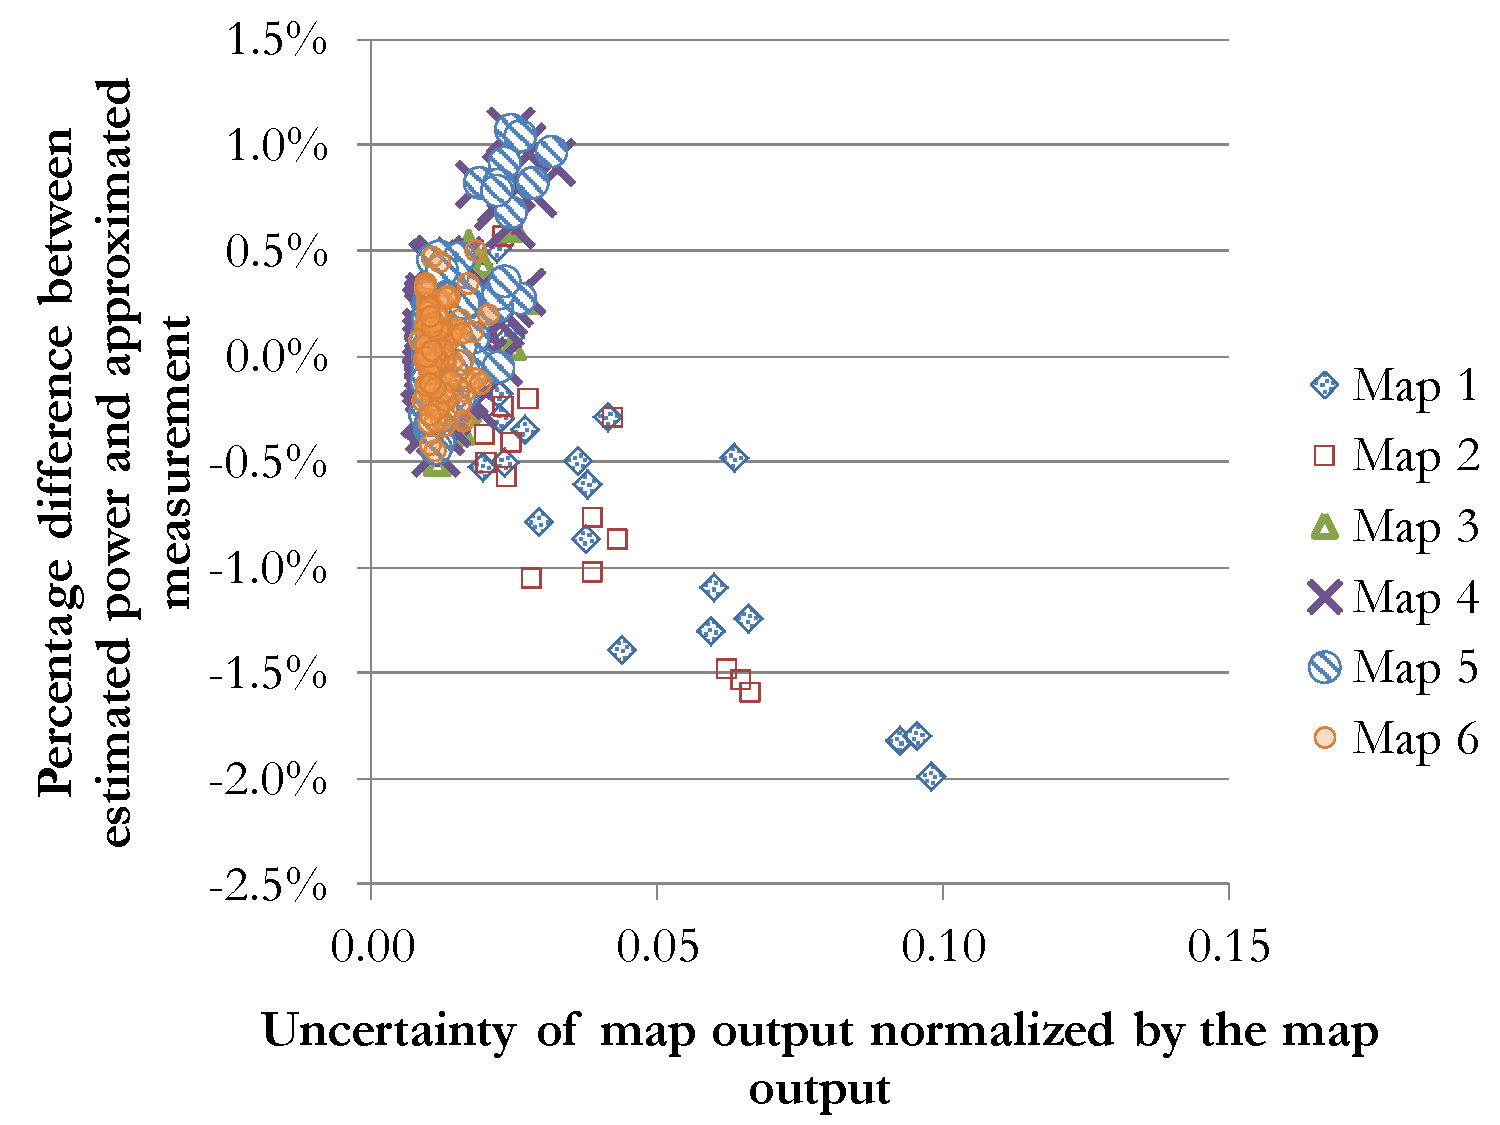
\includegraphics[width=15pc]{rel_diff_to_rel_uncer.pdf}
\caption{\label{fig:rel_uncer}Change of accuracy of maps with output uncertainty in different maps.}
\end{minipage}\hspace{2pc}%
\begin{minipage}{15pc}
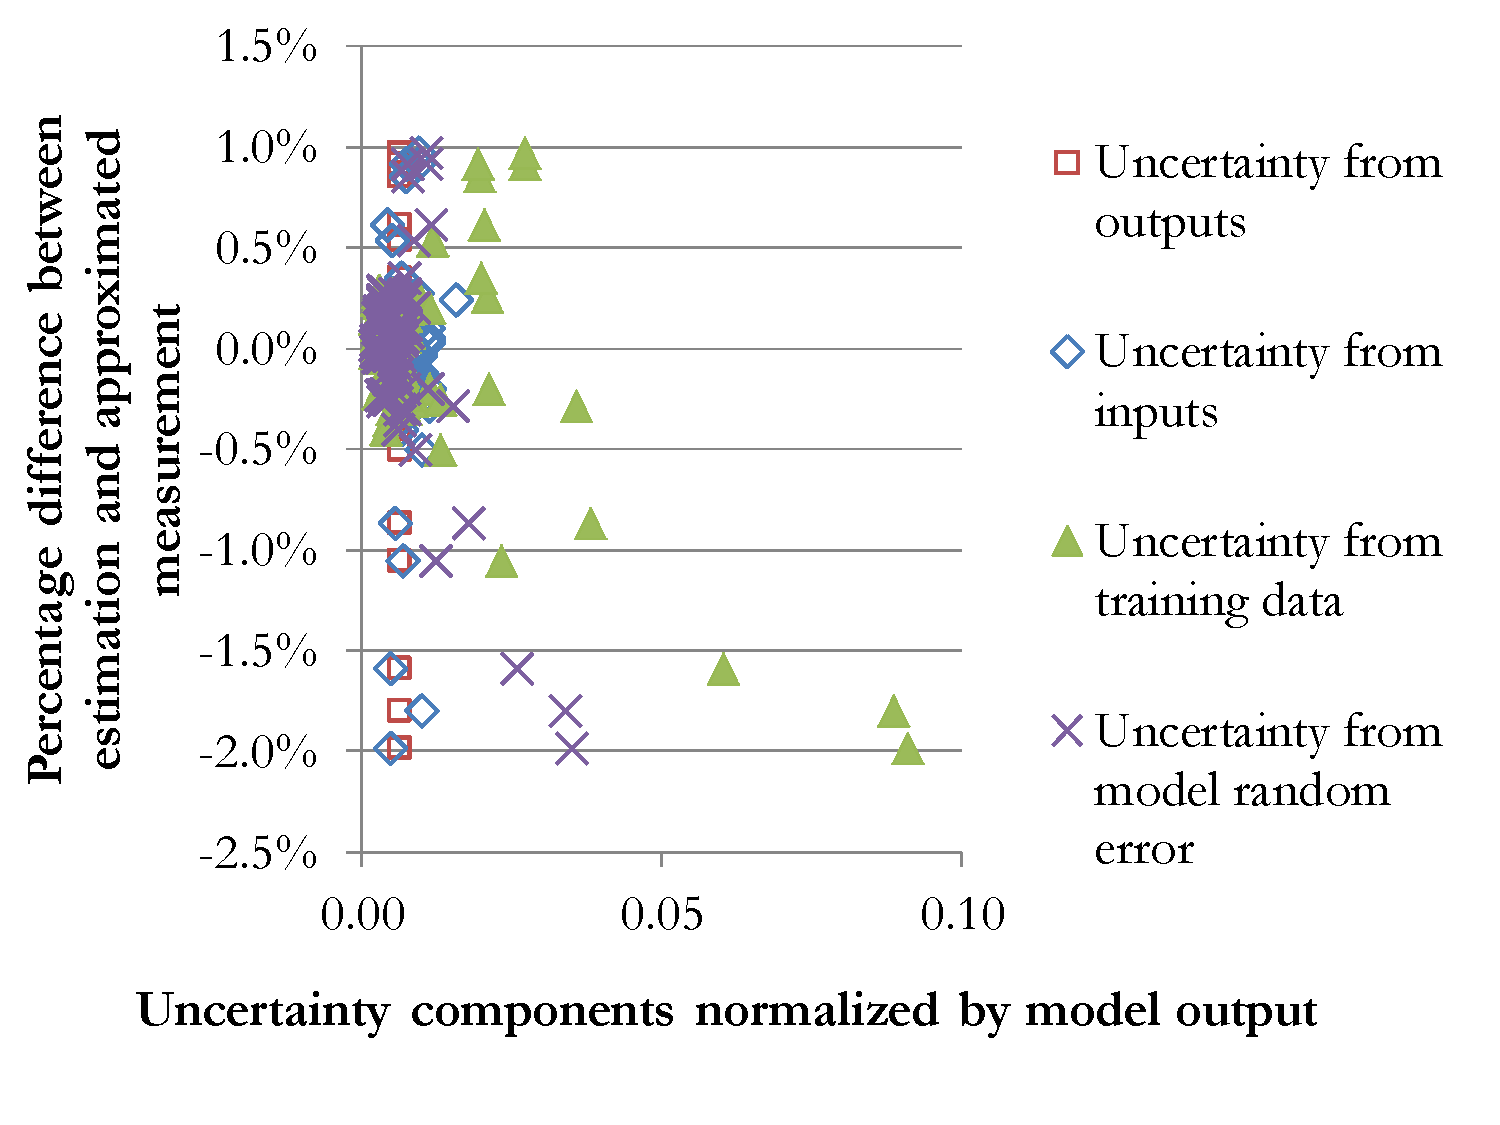
\includegraphics[width=15pc]{rel_diff_to_uncer_comp.pdf}
\caption{\label{fig:uncer_comp}Change of accuracy of maps with different uncertainty components.}
\end{minipage} 
\end{figure}

Figure \ref{fig:rel_uncer} shows that inaccurate map outputs are associated with higher uncertainty and the uncertainty calculation method is a good indicator of the accuracy of the map output. Figure \ref{fig:uncer_comp} shows that the high uncertainty of the inaccurate data points in Figure \ref{fig:rel_uncer} are primarily a result of high uncertainty from model random error and training data.

The increase of uncertainty from model random error with inaccuracy can be explained by the leverage term ${\vec x^T}{({\mathbf{X}}_{train}^T{{\mathbf{X}}_{train}})^{ - 1}}\vec x$ in Eqn. (\ref{eq:uncer_w_model}) which increases as the map extrapolates, and map extrapolation results in lower accuracy. Hence the uncertainty from model random error increase with a decrease of the map accuracy and applicability.

To explain the increase of uncertainty from training data with a decrease of map accuracy in Figure \ref{fig:uncer_comp}, the squared terms in Eqn. (\ref{eq:uncer_w_train}) are labeled as uncertainty from training data per measurement, and their values from two map outputs of Map 1 are plotted as Figures \ref{fig:map_1_low_uncer} and \ref{fig:map_1_high_uncer}.

\begin{figure}[h]
\begin{minipage}{15pc}
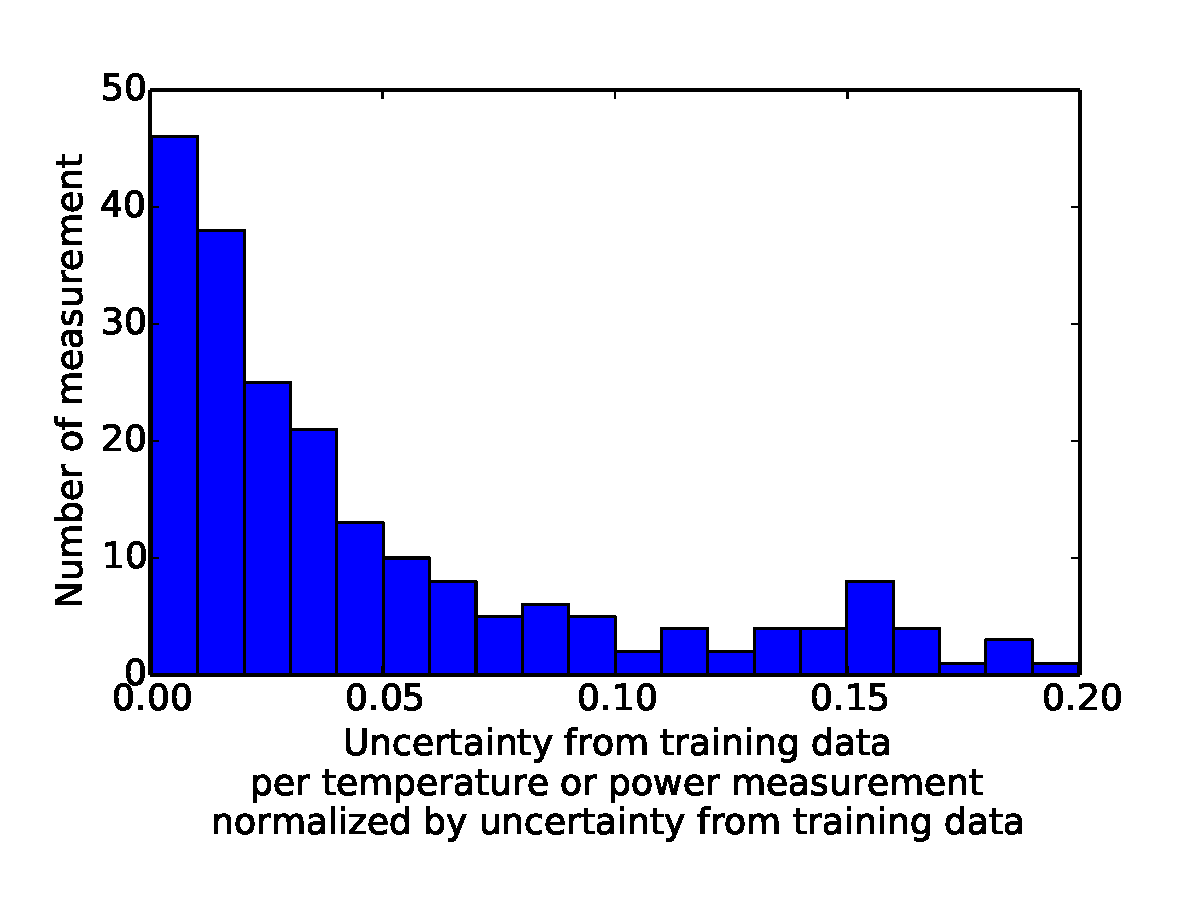
\includegraphics[width=15pc]{Map_1_low_uncer.pdf}
\caption{\label{fig:map_1_low_uncer}Histogram of uncertainty terms in Eqn. (\ref{eq:uncer_w_train}) for $T_{evap} = -1.1^\circ C$ and $T_{cond} = 60.0^\circ C$.}
\end{minipage}\hspace{2pc}%
\begin{minipage}{15pc}
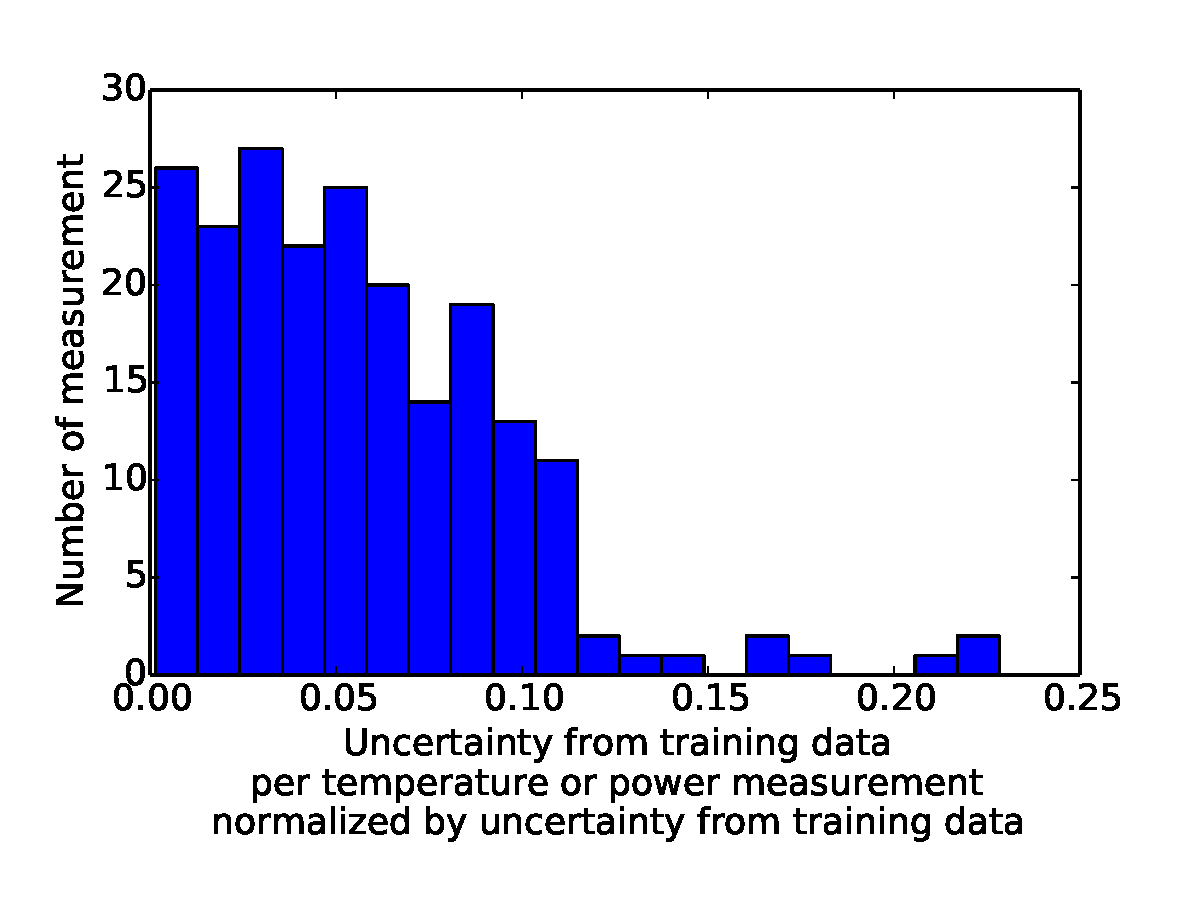
\includegraphics[width=15pc]{Map_1_high_uncer.pdf}
\caption{\label{fig:map_1_high_uncer}Histogram of uncertainty terms in Eqn. (\ref{eq:uncer_w_train}) for $T_{evap} = -28.9^\circ C$ and $T_{cond} = 26.7^\circ C$.}
\end{minipage} 
\end{figure}

Figure \ref{fig:map_1_low_uncer} shows a histogram that is more left-skewed than Figure \ref{fig:map_1_high_uncer}. This is because Figure \ref{fig:map_1_low_uncer} is obtained from a data point inside the training data range of Map 1 (see Figure~\ref{fig:training_envelope}), and the map only needs information from a few data points around $T_{evap} = -1.1^\circ C$ and $T_{cond} = 60.0^\circ C$ to estimate its map output. Hence the estimation does not depend on most of the data points, and their training data uncertainties do not propagate to the map output as shown by Figure \ref{fig:map_1_low_uncer}. 

However, Map 1 extrapolates to the lower left handed corner in Figure \ref{fig:training_envelope} for the condition in Figure \ref{fig:map_1_high_uncer}, and the estimation is significantly affected by multiple data points in the training data. If any of these significant training data points change, the estimation result at this condition will be changed significantly. Hence much more training data points propagate their uncertainty to the map output under the condition in Figure \ref{fig:map_1_high_uncer} than that in Figure \ref{fig:map_1_low_uncer}. This also explains that the uncertainty of training data is a significant component in the extrapolation uncertainty of the map output, and the uncertainty increases as the map applicability and accuracy decrease.
